%%%%%%%%%%%%%%%%%%%%%%%%%%%%%%%%%%%%%%%%%%%%%%%%%%%%%%%%%%%%%%%%%%%%%%
%% Copyright (c) 2016 Carsten Wulff Software, Norway
%% %%%%%%%%%%%%%%%%%%%%%%%%%%%%%%%%%%%%%%%%%%%%%%%%%%%%%%%%%%%%%%%%%%%
%% Created       : wulff at 2016-11-5
%% %%%%%%%%%%%%%%%%%%%%%%%%%%%%%%%%%%%%%%%%%%%%%%%%%%%%%%%%%%%%%%%%%%%
%% This program is free software: you can redistribute it and/or modify
%% it under the terms of the GNU General Public License as published by
%% the Free Software Foundation, either version 3 of the License, or
%% (at your option) any later version.
%%
%% This program is distributed in the hope that it will be useful,
%% but WITHOUT ANY WARRANTY; without even the implied warranty of
%% MERCHANTABILITY or FITNESS FOR A PARTICULAR PURPOSE.  See the
%% GNU General Public License for more details.
%%
%% You should have received a copy of the GNU General Public License
%% along with this program.  If not, see <http://www.gnu.org/licenses/>.
%%%%%%%%%%%%%%%%%%%%%%%%%%%%%%%%%%%%%%%%%%%%%%%%%%%%%%%%%%%%%%%%%%%%%%
%\documentclass[final,11pt]{IEEEtran}
\documentclass[crop,border=0pt]{standalone}
\usepackage{times}


%\usepackage{placeins}
\usepackage{upgreek}
\usepackage{amssymb,amsmath}
\usepackage{cite}
\usepackage{verbatim}
\usepackage{listings}
\usepackage{xcolor}
\usepackage{flafter}
\usepackage{booktabs}
\usepackage{url}
\usepackage{ textcomp }

\hyphenation{op-tical net-works semi-conduc-tor}


% -JSON styel

%\definecolor{darkGreen}{rgb}{0,0.2097,0}
%\newcommand{\myfigwidth}{\linewidth}
%\newcommand{\myfigwidtha}{\linewidth}
%\newcommand{\myfigwidthl}{\textwidth}
%\newcommand{\myfigwidthc}{0.6\linewidth}


\newcommand{\myfigwidtha}{3.3in}
\newcommand{\myfigwidthl}{7in}
\newcommand{\myfigwidthc}{2in}
%\newcommand{\myfigwidthe}{3.2in}
%\newcommand{\myfigwidthb}{5in}

\newcommand{\myfigname}{fig_}
\newcommand{\reg}[2]{{\figurename} \ref{#1}(#2)}
\newcommand{\req}[1]{{\figurename} \ref{#1}}
%\newcommand{\myeqname}{eq:}
%\newcommand{\req}[1]{(\ref{\myeqname#1})}

\definecolor{armygreen}{rgb}{0, 0.5, 0}
\newcommand{\missing}[1]{{ #1}}
\newcommand{\edit}[1]{{ #1}}
\newcommand{\secedit}[1]{{ #1}}
\newcommand{\deleted}[1]{{ #1}}
\newcommand{\moved}[1]{{ #1}}

%\newcommand{\missing}[1]{{\color{red} #1}}
%\newcommand{\edit}[1]{{\color{red} #1}}
%\newcommand{\secedit}[1]{{\color{armygreen} #1}}
%\newcommand{\deleted}[1]{{\color{violet} #1}}
%\newcommand{\moved}[1]{{\color{blue} #1}}

\newcommand{\SD}{Sigma-Delta }
\newcommand{\eqn}[1]{
  \begin{math}
    #1
  \end{math}}

\newcommand\JSONnumbervaluestyle{\color{blue}}
\newcommand\JSONstringvaluestyle{\color{red}}



\newif\ifcolonfoundonthisline

\makeatletter

\lstdefinestyle{json}
{
  showstringspaces    = false,
  keywords            = {false,true},
  alsoletter          = 0123456789.,
  morestring          = [s]{"}{"},
  stringstyle         = \ifcolonfoundonthisline\JSONstringvaluestyle\fi,
  MoreSelectCharTable =%
  \lst@DefSaveDef{`:}\colon@json{\processColon@json},
  basicstyle          = \fontsize{7}{7}\ttfamily,
  keywordstyle        = \fontsize{7}{7}\ttfamily\bfseries,
}

% flip the switch if a colon is found in Pmode
\newcommand\processColon@json{%
  \colon@json%
  \ifnum\lst@mode=\lst@Pmode%
  \global\colonfoundonthislinetrue%
  \fi
}

\lst@AddToHook{Output}{%
  \ifcolonfoundonthisline%
  \ifnum\lst@mode=\lst@Pmode%
  \def\lst@thestyle{\JSONnumbervaluestyle}%
  \fi
  \fi
  % override by keyword style if a keyword is detected!
  \lsthk@DetectKeywords%
}

% reset the switch at the end of line
\lst@AddToHook{EOL}%
{\global\colonfoundonthislinefalse}

\makeatother

% \lstset{  basicstyle=\tiny}

% \lstset{
% basicstyle=\fontsize{11}{13}\selectfont\ttfamily
% }


\lstset{language=Java}




%\usepackage[paperwidth=\maxdimen,paperheight=\maxdimen]{geometry}


\usepackage{tikz,pgfplots}
\usepackage{ifthen}
\usepackage{calc}
\usetikzlibrary{patterns}
%\usepackage[tightpage,active]{preview}
\usetikzlibrary{circuits.logic.US}
\usetikzlibrary{circuits.ee.IEC}
\usepgflibrary{shapes.arrows}
\usepgflibrary{arrows}
\usepackage{circuitikz}


% circuitikz draws bipole outlines (resistors, diodes, capacitors) at
% bipoles/thickness times the ambient line width, and the default is 2.
% That makes a circuitikz resistor visibly heavier than the wire it sits
% on, and heavier than the hand rolled zig-zag in ckt_lib.tex. One is the
% house width: everything is drawn at the environment's own thickness.
% Arrow tips: one filled tip everywhere, set through the '>' knob so a
% figure only ever writes ->, <- or <->. Latex (from arrows.meta)
% scales with the line width, so it stays in proportion if a drawing
% is ever set thicker or thinner than the house 'thick'.
\usetikzlibrary{arrows.meta}
\tikzset{>={Latex}}

\ctikzset{bipoles/thickness=1}
\ctikzset{tripoles/mos style/arrows}
\ctikzset{tripoles/pmos style/emptycircle}
%\PreviewEnvironment{circuitikz}
\pagestyle{empty}


\tikzstyle{cicfill}=[minimum size=1.4em]
\tikzstyle{stuff_fill}=[rectangle,fill=white,minimum size=1.4em]

\newcommand{\grayOne}{0.3 }
\newcommand{\grayTwo}{0.15 }
\newcommand{\grayThree}{0.26 }
\newcommand{\grayFour}{0.41 }
\newcommand{\grayFive}{0.61 }
\newcommand{\graySix}{0.85 }

%- Gray tone
%\definecolor{active}{rgb}{\graySix,\graySix,\graySix}
%\definecolor{poly}{rgb}{\grayFive,\grayFive,\grayFive}
%\definecolor{contact}{rgb}{\graySix,\graySix,\graySix}
%\definecolor{mOne}{rgb}{\grayFour,\grayFour,\grayFour}
%\definecolor{mTwo}{rgb}{\graySix,\graySix,\graySix}
%\definecolor{mThree}{rgb}{\grayThree,\grayThree,\grayThree}
%\definecolor{mFour}{rgb}{\grayTwo,\grayTwo,\grayTwo}

\definecolor{grey}{rgb}{1,1,1}
\definecolor{lightgrey}{rgb}{\grayFour,\grayFour,\grayFour}
\definecolor{active}{rgb}{0.4,1,0.6}
\definecolor{poly}{rgb}{1.0,0.5,0.5}
\definecolor{cut}{rgb}{0.91,0.91,0}
\definecolor{mOne}{rgb}{0.36,0.36,1}
\definecolor{mTwo}{rgb}{0.655,0.655,0}
\definecolor{mThree}{rgb}{0.3,1,1}
\definecolor{mFour}{rgb}{0,0.2097,0}
\begin{document}


% All-digital PLL with a bang-bang phase detector for steady state, after
% the architecture in Cole Nielsen's master's thesis work (NTNU, 2020).
% The reference CLK clocks the phase error logic, which compares it with a
% synchronous counter clocked by the DCO output, and clocks a D flip-flop
% that samples the output as a bang-bang phase detector (BB-PD). A mux
% picks the multi-bit phase error during lock-in and the one-bit BB-PD
% once the steady-state detector (SS Detect) says the loop has settled;
% the same signal disables the phase error logic through an inverter and
% enables the BB-PD. The loop filter is proportional (a0) plus a delayed
% path (z^-1, a1), followed by an integrator (adder with z^-1 feedback)
% whose state the calibration engine can load. The DCO calibration engine
% gets the frequency error from the offset estimator, the difference of
% the phase error and its value n cycles earlier, and sets the DCO coarse
% word, drives the fine word directly through the second mux while
% calibrating, and preloads the loop filter state before handing over.
% Drawn in black, with the subsystems as dashed boxes, so it matches the
% rest of the book.

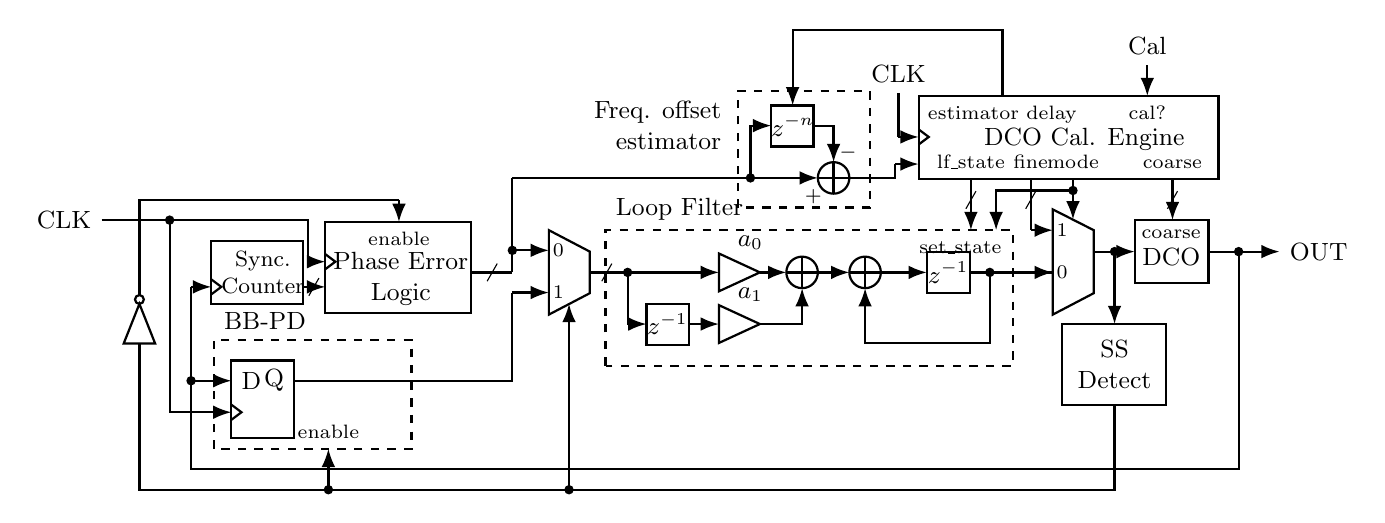
\begin{tikzpicture}[thick, x=0.8cm, y=0.8cm, font=\small]

  \tikzset{bus/.pic={\draw[thin] (-0.08,-0.14) -- (0.08,0.14);},
           sm/.style={font=\scriptsize}}

  % reference clock
  \node[anchor=east] at (0.3,4.43) {CLK};
  \draw (0.3,4.43) -- (3.58,4.43) -- (3.58,3.77);
  \draw[->] (3.58,3.77) -- (3.85,3.77);
  \fill (1.38,4.43) circle (0.075);
  \draw[->] (1.38,4.43) -- (1.38,1.38) -- (2.36,1.38);

  % synchronous counter and phase error logic
  \draw (2.04,3.10) rectangle (3.5,4.10);
  \node[align=center, font=\footnotesize] at (2.86,3.6) {Sync.\\Counter};
  \draw (2.04,3.25) -- (2.2,3.37) -- (2.04,3.49);
  \draw (3.85,2.95) rectangle (6.17,4.4);
  \node[align=center] at (5.05,3.5) {Phase Error\\Logic};
  \draw (3.85,3.65) -- (4.01,3.77) -- (3.85,3.89);
  \node[sm, anchor=north] at (5.02,4.4) {enable};
  \draw[->] (3.5,3.37) -- (3.85,3.37);
  \pic at (3.67,3.37) {bus};

  % bang-bang phase detector
  \draw[dashed] (2.08,0.8) rectangle (5.22,2.53);
  \node[anchor=south west] at (2.08,2.53) {BB-PD};
  \draw (2.36,0.97) rectangle (3.36,2.2);
  \node[anchor=west] at (2.36,1.88) {D};
  \node[anchor=east] at (3.36,1.88) {Q};
  \draw (2.36,1.26) -- (2.52,1.38) -- (2.36,1.5);
  \node[sm, anchor=south] at (3.9,0.8) {enable};

  % input mux: phase error (0) or BB-PD (1)
  \draw (7.4,4.27) -- (8.05,3.93) -- (8.05,3.27) -- (7.4,2.93) -- cycle;
  \node[sm] at (7.55,3.95) {0};
  \node[sm] at (7.55,3.28) {1};
  \draw (6.17,3.6) -- (6.82,3.6);
  \pic at (6.5,3.6) {bus};
  \fill (6.82,3.95) circle (0.075);
  \draw (6.82,3.6) -- (6.82,5.1);
  \draw[->] (6.82,3.95) -- (7.4,3.95);
  \draw (3.36,1.88) -- (6.82,1.88) -- (6.82,3.28);
  \draw[->] (6.82,3.28) -- (7.4,3.28);

  % loop filter
  \draw[dashed] (8.3,2.12) rectangle (14.77,4.27);
  \node[anchor=south west] at (8.3,4.27) {Loop Filter};
  \draw (8.05,3.6) -- (8.65,3.6);
  \pic at (8.32,3.6) {bus};
  \fill (8.65,3.6) circle (0.075);
  \draw (10.1,3.9) -- (10.75,3.6) -- (10.1,3.3) -- cycle;
  \node[anchor=south] at (10.6,3.8) {$a_0$};
  \draw[->] (8.65,3.6) -- (10.1,3.6);
  \draw (8.95,2.45) rectangle (9.62,3.1);
  \node at (9.28,2.78) {$z^{-1}$};
  \draw[->] (8.65,3.6) -- (8.65,2.78) -- (8.95,2.78);
  \draw (10.1,3.08) -- (10.75,2.78) -- (10.1,2.48) -- cycle;
  \node[anchor=south] at (10.6,2.98) {$a_1$};
  \draw[->] (9.62,2.78) -- (10.1,2.78);
  \draw (11.42,3.6) circle (0.25);
  \draw (11.17,3.6) -- (11.67,3.6) (11.42,3.35) -- (11.42,3.85);
  \draw[->] (10.75,3.6) -- (11.17,3.6);
  \draw[->] (10.75,2.78) -- (11.42,2.78) -- (11.42,3.35);
  \draw (12.42,3.6) circle (0.25);
  \draw (12.17,3.6) -- (12.67,3.6) (12.42,3.35) -- (12.42,3.85);
  \draw[->] (11.67,3.6) -- (12.17,3.6);
  \draw (13.4,3.27) rectangle (14.08,3.93);
  \node at (13.74,3.6) {$z^{-1}$};
  \draw[->] (12.67,3.6) -- (13.4,3.6);
  \draw (14.08,3.6) -- (15.4,3.6);
  \fill (14.4,3.6) circle (0.075);
  \draw[->] (14.4,3.6) -- (14.4,2.48) -- (12.42,2.48) -- (12.42,3.35);
  \node[sm, anchor=north east] at (14.75,4.25) {set\_state};

  % output mux: loop filter (0) or calibration fine word (1)
  \draw (15.4,4.6) -- (16.05,4.27) -- (16.05,3.27) -- (15.4,2.93) -- cycle;
  \node[sm] at (15.55,4.27) {1};
  \node[sm] at (15.55,3.6) {0};
  \draw[->] (15.0,3.6) -- (15.4,3.6);

  % DCO and output
  \draw (16.7,3.43) rectangle (17.87,4.43);
  \node at (17.28,3.85) {DCO};
  \node[sm, anchor=north] at (17.28,4.43) {coarse};
  \draw[->] (16.05,3.93) -- (16.7,3.93);
  \fill (16.38,3.93) circle (0.075);
  \draw[->] (17.87,3.93) -- (19.0,3.93) node[anchor=west] {OUT};
  \fill (18.35,3.93) circle (0.075);

  % the output clocks the counter and is sampled by the BB-PD
  \draw (18.35,3.93) -- (18.35,0.48) -- (1.72,0.48) -- (1.72,3.37);
  \draw[->] (1.72,3.37) -- (2.04,3.37);
  \fill (1.72,1.88) circle (0.075);
  \draw[->] (1.72,1.88) -- (2.36,1.88);

  % steady-state detect selects the BB-PD and disables the phase error logic
  \draw (15.55,1.5) rectangle (17.2,2.78);
  \node[align=center] at (16.38,2.14) {SS\\Detect};
  \draw[->] (16.38,3.93) -- (16.38,2.78);
  \draw (16.38,1.5) -- (16.38,0.15) -- (0.9,0.15) -- (0.9,2.47);
  \fill (7.72,0.15) circle (0.075);
  \draw[->] (7.72,0.15) -- (7.72,3.1);
  \fill (3.9,0.15) circle (0.075);
  \draw[->] (3.9,0.15) -- (3.9,0.8);
  \draw (0.65,2.47) -- (1.15,2.47) -- (0.9,3.1) -- cycle;
  \draw (0.9,3.17) circle (0.07);
  \draw (0.9,3.24) -- (0.9,4.75) -- (5.02,4.75);
  \draw[->] (5.02,4.75) -- (5.02,4.4);

  % frequency offset estimator: phase error minus its value n cycles ago
  \draw[dashed] (10.4,4.63) rectangle (12.5,6.48);
  \node[anchor=north east, align=right] at (10.3,6.48) {Freq. offset\\estimator};
  \draw (6.82,5.1) -- (10.6,5.1);
  \fill (10.6,5.1) circle (0.075);
  \draw[->] (10.6,5.1) -- (11.67,5.1);
  \draw (11.92,5.1) circle (0.25);
  \draw (11.67,5.1) -- (12.17,5.1) (11.92,4.85) -- (11.92,5.35);
  \node[sm] at (11.6,4.8) {$+$};
  \node[sm] at (12.15,5.5) {$-$};
  \draw (10.93,5.6) rectangle (11.6,6.25);
  \node at (11.27,5.93) {$z^{-n}$};
  \draw[->] (10.6,5.1) -- (10.6,5.93) -- (10.93,5.93);
  \draw[->] (11.6,5.93) -- (11.92,5.93) -- (11.92,5.35);
  \draw (12.17,5.1) -- (12.9,5.1) -- (12.9,5.32);
  \draw[->] (12.9,5.32) -- (13.27,5.32);

  % DCO calibration engine
  \draw (13.27,5.08) rectangle (18.03,6.4);
  \node at (15.9,5.72) {DCO Cal. Engine};
  \draw (13.27,5.63) -- (13.43,5.75) -- (13.27,5.87);
  \node[anchor=south] at (12.95,6.45) {CLK};
  \draw (12.95,6.45) -- (12.95,5.75);
  \draw[->] (12.95,5.75) -- (13.27,5.75);
  \foreach \x/\n in {14.1/lf\_state, 15.05/fine, 15.72/mode, 17.3/coarse} {
    \node[sm, anchor=south] at (\x,5.08) {\n};
  }
  \node[sm, anchor=north] at (14.6,6.4) {estimator delay};
  \node[sm, anchor=north] at (16.9,6.4) {cal?};
  \draw[->] (14.6,6.4) -- (14.6,7.45) -- (11.27,7.45) -- (11.27,6.25);
  \draw[<-] (16.9,6.4) -- (16.9,6.9) node[anchor=south] {Cal};
  \draw[->] (14.1,5.08) -- (14.1,4.27);
  \pic at (14.1,4.75) {bus};
  \draw (15.05,5.08) -- (15.05,4.27);
  \draw[->] (15.05,4.27) -- (15.4,4.27);
  \pic at (15.05,4.75) {bus};
  \draw[->] (15.72,5.08) -- (15.72,4.44);
  \fill (15.72,4.9) circle (0.075);
  \draw[->] (15.72,4.9) -- (14.5,4.9) -- (14.5,4.27);
  \draw[->] (17.3,5.08) -- (17.3,4.43);
  \pic at (17.3,4.75) {bus};

\end{tikzpicture}
\end{document}
